\documentclass[bigger]{beamer}
\useinnertheme{circles}
\usefonttheme[onlymath]{serif}
\usefonttheme{structurebold}
\setbeamertemplate{navigation symbols}{}
\usepackage{xcolor}
\setbeamercolor{highlight block}{bg=gray}

\usepackage{tikz}
\usetikzlibrary{
    automata,%
    positioning,%
    calc,%
    decorations,%
    decorations.pathmorphing%
}
\usepackage{tkz-graph}
\newcommand{\qlr}[2]{\ensuremath{\begin{matrix}#1\cr\begin{aligned}\hline #2\end{aligned}\end{matrix}}}
\newcommand{\q}[1]{\mathbf{#1}}
\newcommand{\isep}{~,~}

\usepackage[T1]{fontenc}
\usepackage[utf8]{inputenc}
\usepackage[normalem]{ulem} % To strikeout
\usepackage{commath}

\newcommand{\naf}{\ensuremath{\sim\!\!}}

\title{Probabilistic Answer Set Programming}
\subtitle{A Research Draft}
\author{Francisco Coelho}
\institute[\texttt{fc@uevora.pt}]{
    NOVA LINCS \&\\
    High Performance Computing Chair \&\\
    Departamento de Informática, Universidade de Évora
}

\begin{document}
    \begin{frame}[plain]
        \titlepage
    \end{frame}
    
    \section*{Motivation}

    \begin{frame}
        \frametitle{In short}
    
        \begin{itemize}
            \item Use \textbf{logic programs} to formalize knowledge.
            \begin{itemize}
                \item logic program = formula = model.
                \item \textbf{Observations} not always agree with such models --- errors may result from sensors or from a wrong or incomplete model.
            \end{itemize}
            \item We can associate \textbf{quantities} to formulas and sub-formulas.
            \begin{itemize}
                \item And define how observations \textbf{update} those quantities.
            \end{itemize}            
            \item Adequate quantities and updates might be used to \textbf{interpret or evaluate the model} \emph{e.g.} define a joint distribution or measure the accuracy of a clause. 
        \end{itemize}            
    \end{frame}

    % \begin{frame}
    %     \frametitle{Plan}
    %     \begin{itemize}
    %         \item Use \textbf{answer set programs} as a logic programming language.
    %         \item Define the effect of an \textbf{observation} on quantities associated to clauses and their parts.
    %         \item Later, use those numbers to define \textbf{probabilistic interpretations} or \textbf{performance quantities} of a formula, clauses and atoms.
    %     \end{itemize}
    % \end{frame}
    
    \section{Development}
    
    \begin{frame}
        \tableofcontents[currentsection]
    \end{frame}

    % \begin{frame}
    %     \frametitle{The seed on an idea}
    %     We want to define the \textbf{joint distribution} of the stable models.
    %     \begin{enumerate} 
    %         \item A \textbf{boolean random variable} can be described by a disjunction $a; \neg a$.
    %         \item This ASP program has two stable models: $a$ and $\neg a$.
    %         \item A program with $n$ such facts $a_i; \neg a_i$ has $2^n$ stable models, the distinct combinations of those choices. 
    %         \item \textbf{If each $a_i$ has probability $p_i$ then the probability of a stable model $W$ would be} $$P(W) = \prod_{a_i \in W}p_i \prod_{\neg a_i \in W} (1 - p_i).$$            
    %     \end{enumerate}        
    %     \pause
    %     \begin{alertblock}{But this is wrong.}
    %         Even assuming that those facts are marginally independent --- which we will do.
    %     \end{alertblock}
    % \end{frame}

    \begin{frame}{Problem 1: Probabilities}
        The stable models of $c_1 \wedge c_2$ where
        $$        
        \begin{aligned}
            c_1 &: b \vee \neg b\\
            c_2 &: h_1 \vee h_2 &\leftarrow b
        \end{aligned}
        $$
        are $$\set{\neg b}, \set{b, h_1}~\text{and}~\set{b, h_2}.$$  

        \begin{block}{Associate quantities to clauses and update them with observations.}        
            \onslide*<1>{
                Then compute:
                \begin{itemize}
                    \item The probability of a stable model. 
                    \item The probability of an atom.
                    \item The joint distribution of all atoms.
                \end{itemize}
            }
            \onslide*<2>{
                \begin{itemize}
                    \item How to \textbf{match} an observation $z$ with a clause case $h_i,b$?
                    \item How do observations \textbf{update} the probabilities?
                    \item Is this enough to compute the \textbf{joint distribution of the atoms}?
                \end{itemize}
            }
        \end{block}    
    \end{frame}

    \begin{frame}
        \frametitle{Matching observations and sub-formulas}

        \begin{itemize}
            \item An \alert{observation} is a subset of the literals\footnote{The set of atoms, $a$, of the program and their classic negations, $\neg a$.} from a program.
            \item A \alert{consistent} observation has no subset $\set{p, \neg p}$.
            \item A \emph{consistent} observation $z$ is \alert{relevant} for the clause $h \leftarrow b$ if $b \subseteq z$.
            \item A disjunctive clause $$h_1 \vee \cdots \vee h_n \leftarrow b_1 \wedge \cdots \wedge b_m$$ has $n$ \alert{cases}: $\set{h_i, b_1, \ldots, b_m}, i = 1:n$.
            \item The \emph{consistent} observation $z$ and the case $\set{h, b_{1:n}}$  \alert{match} if 
            $\set{h, b_{1:n}} \subseteq z$.     
        \end{itemize}
        The above definitions apply to \textbf{facts}, $m=0$, and \textbf{constraints}, $n=0$.
    \end{frame}

    \begin{frame}
        \frametitle{Counters and updates}
        A consistent observation \textbf{relevant} for a clause $h_1 \vee \cdots \vee h_n \leftarrow b$ should \textbf{increase the probability of matched cases}.
        \begin{block}{Counters and updates}
            \onslide*<1>{
            \begin{enumerate}
                \item Associate \textbf{counters}, $u, r, n$, to clauses $h \leftarrow b$.
                \item Associate a \textbf{counter}, $m_i$, to cases $h_i, b$.
                \item \textbf{Initial} values result from \emph{prior} knowledge.
                \item Each \emph{consistent} observation \textbf{increments}:
                \begin{itemize}
                    \item The $u$ counters of relevant \alert{u}nmatched clauses (no matched cases).
                    \item The $r$ counters of \alert{r}elevant clauses. 
                    \item The $n$ counters of \alert{n}ot relevant clauses.
                    \item The $m_i$ counters of \alert{m}atched cases $h_i, b$.
                    \item Clause counters must verify $r \leq u + \sum_i m_i$.
                \end{itemize}
            \end{enumerate}  
            }
            \onslide*<2>{
                \begin{itemize}
                    \item Literals must be explicitly observed: $\neg b \not= \naf b$.
                    \item Counters relate a clause structure with observations.
                    \item So far stable models had no role. 
                \end{itemize}
            }
        \end{block}
    \end{frame}

    \begin{frame}
        \frametitle{Counters and updates: An example}
        Given the following clauses with \alert{annotated counters},
        $$        
        \begin{aligned}
            %&H \leftarrow B&&\text{counters:}~ m_{1:n} ; u, r, n \\
            &b \vee \neg b &&\text{counters:}~ 7, 2 ; 3, 12, 0 \\
            &h_1 \vee h_2 \leftarrow b  &&\text{counters:}~ 4, 3 ; 2, 6, 5
        \end{aligned}
        $$
        \onslide*<2>{
            \begin{columns}[t]
                \begin{column}{0.5\textwidth}                    
                \begin{block}{Counters of $b \vee \neg b$}\small
                    $0$ observations where not relevant (because the body is $\top$); 
                    
                    There where $12$ relevant observations; 
                    
                    Of those, $b$ was matched by $7$, $\neg b$ by $2$ and $3$ observations matched neither ($\models\naf b, \naf \neg b$).
                \end{block}
                \end{column}
                \begin{column}{0.5\textwidth}                    
                \begin{block}{Counters of $h_1 \vee h_2 \leftarrow b$}\small
                    There where $11 = 6 + 5$ observations, $6$ relevant to this clause; 
                    
                    From these, $4$ matched $h_1$, $3$ matched $h_2$ and $2$ matched no case.
                \end{block}
                \end{column}
            \end{columns}
        }
        \onslide*<3>{
        \begin{block}{What can be computed?}
            \begin{itemize}
                \item $P(\neg b) = \frac{2}{12}$ because $\neg b$ matched $2$ of $12$ relevant observations.
                \item $P(h_1 | b) = \frac{4}{6}$ because $h_1, b$ matched $4$ of $6$ relevant observations.
                \item \alert{$P(b)$ needs further information}. 
                \begin{itemize}
                    \item \emph{E.g.} \textbf{assuming independent observations},
                    $$P(b) = \frac{7 + 6}{12 + 0 + 6 + 5}.$$ 
                \end{itemize}                
            \end{itemize}            
        \end{block}}
        \onslide*<4>{
        \begin{block}{What can be computed? --- assuming independent observations}
            \begin{itemize}
                \item $P(b) + P(\neg b) = \frac{13}{23} + \frac{2}{12} \approx 0.73 < 1$ because some observations have neither $b$ nor $\neg b$.
                \item $P(h_1, b) = P(h_1 | b) P(b) = \frac{4}{6}\frac{13}{23}$ from above.
                \item $P(h_2, b) = P(h_2 | b) P(b)$ is analogous.
                \item \alert{But not \emph{e.g.} $P(h_1 | \neg b)$} because no clause relates $h_1$ and $\neg b$.
            \end{itemize}            
        \end{block}}
        \onslide*<5->{
            \begin{block}{Also\ldots}
                \onslide*<5>{Counters are local to clauses and, for distinct clauses, may result from distinct sources. \emph{E.g. the relevant counter of $h_1 \vee h_2 \leftarrow b$ and the match counter of $b$ in $b \vee \neg b$.}}
                \onslide*<6>{Some observations may have neither $b$ nor $\neg b$ so: $$P(b) + P(\neg b) < 1.$$}
                \onslide*<7>{Assuming independent observations, since $h_1$ and $h_2$ are not independent, $$\sum_m P(m) > 1.$$}
                \onslide*<8>{What's missing to define the \alert{joint distribution} $$P(H_1, H_2, B)?$$}
            \end{block}
        }
        \onslide*<8->{
            \begin{block}{The joint distribution, according to the clauses}
                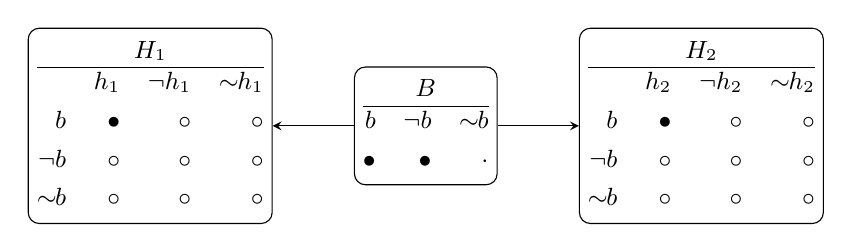
\begin{tikzpicture}[node distance=35mm, ->, >=stealth, state/.style={draw, rounded corners}]\small
                    \node (B) [state] {\qlr{B}{
                        b && \neg b && \naf b \cr
                        \bullet && \bullet && \cdot
                        }};
                    \node (H1) [state, left of=B] {
                        \qlr{H_1}{
                            ~ && h_1 && \neg h_1 && \naf h_1 \cr
                            b && \bullet && \circ  && \circ \cr
                            \neg b && \circ  && \circ  && \circ \cr
                            \naf b && \circ  && \circ  && \circ 
                        }
                    };
                    \node (H2) [state, right of=B] {
                        \qlr{H_2}{
                            ~ && h_2 && \neg h_2 && \naf h_2 \cr
                            b && \bullet && \circ  && \circ \cr
                            \neg b && \circ  && \circ  && \circ \cr
                            \naf b && \circ  && \circ  && \circ 
                        }
                    };
                    \path
                        (B) edge (H1)
                        (B) edge (H2)
                    ;
                \end{tikzpicture}
            \end{block}
        }
    \end{frame}
    
    \begin{frame}
        \frametitle{Shortcomming 2: Default Negation}
    
        \begin{itemize}
            \item How to deal with rules with $\naf a$ parts?
            \item Should missing elements on observations be replaced with $\naf a$ atoms?
        \end{itemize}
    \end{frame}
    \section{Conclusions}
    
    \begin{frame}
        \tableofcontents[currentsection]
    \end{frame}
    
    \section*{Background Material}
    
    \begin{frame}
        \Huge Background Material
    \end{frame}

    \begin{frame}{Machine Learning}
        Models are numeric functions: $y \approx f_\theta(x),~\theta_i, x_j, y\in\mathbf{R}$.
        \begin{itemize}
            \item Amazing achievements.
            \item Noise tolerant.
            \item (as of today) Huge enterprise funding .
        \end{itemize}
        but
        \begin{itemize}
            \item (essentially) Academically solved.
            \item Models trained from ``large'' amounts of samples.
            \item Hard to add background knowledge.
            \item Models are hard to interpret.
            \item Single table, independent rows assumption.
        \end{itemize}
    \end{frame}
    
    \begin{frame}{Inductive Logic Programming}
        Models are logic program: $p_\theta(x, y),~\theta_i, x_j, y\in{\cal A}$.
        \begin{itemize}
            \item Amazing achievements, at scale.
            \item Models trained from ``small'' amounts of samples.
            \item Compact, readable models.
            \item Background knowledge is easy to incorporate and edit.
        \end{itemize}
        but
        \begin{itemize}
            \item as of today, Little enterprise commitment.
            \item as of today, Mostly academic interest.
            \item Noise sensitive.
        \end{itemize}
    \end{frame}

    \begin{frame}{Distribution Semantics}
        Assigns probability to (marginally independent) facts and derives probability of ground propositions.

        Let $F$ be set of facts, $S\subseteq F$, $R$ a set of definite clauses and $p$ a proposition:
        $$\small
        \begin{aligned}
            P_F(S) &= \prod_{f \in S} P(f) \prod_{f \not\in S} \left(1 - P(f) \right) \cr
            P(W) &= \sum_{S \subseteq F :~W=M(S\cup R)} P_F(S) \cr
            P(p) &= \sum_{S :~ S\cup R ~\vdash~ p} P_F(S) = \sum_{W :~ p\in W} P(W)
        \end{aligned}
        $$
        \begin{itemize}
            \item Amazing achievements, at scale.
            \item Lots of tools and research.
            \item The best of both ``worlds''?
        \end{itemize}
        
    \end{frame}

    \begin{frame}{Answer Set Programming}
        A program defines stable models.  
        \begin{itemize}
            \item Pure declarative language, unlike Prolog.
            \item Uses \emph{generate \& test} methods instead of proofs.
            \item Uses both default $\sim\!p$ and classical negation $\neg p$.
            \item Clauses can be disjunctive $a \vee b \leftarrow c \wedge d$.
        \end{itemize}
    \end{frame}

    \begin{frame}{ASP definitions}
        \begin{itemize}
            \item An \textbf{atom} is $r(t_1, \ldots t_n)$ where
            \begin{itemize}
                \item $r$ is a $n$-ary predicate symbol.
                \item each $t_i$ is a constant or a variable.
            \end{itemize}
            \item A \textbf{ground atom} has no variables.
            \item A \textbf{literal} is either an atom $a$ or a negated atom $\neg a$.
            \item An \textbf{ASP Program} is a set of \textbf{rules} such as $h_1 \vee \cdots \vee h_m \leftarrow b_1 \wedge \cdots \wedge b_n$ where
            \begin{itemize}
                \item Each $h_i$ is a literal, $a$ or $\neg a$.
                \item Each $b_j$ is a literal like above or preceded by $\naf~$.
                \item $m + n > 0$.
            \end{itemize}
            \item The \textbf{head} of such rule is $h_1 \vee \cdots \vee h_m$.
            \item The \textbf{body} of such rule is $b_1 \wedge \cdots \wedge b_n$.
            \item Each $b_i$ is a \textbf{subgoal}.
        \end{itemize}
    \end{frame}

    \begin{frame}{ASP definitions \hfill(cont.)}
        \begin{itemize}\setcounter{enumi}{7}
            \item A \textbf{non-disjunctive rule} has $m \leq 1$.
            \item A \textbf{normal rule} has $m = 1$.
            \item A \textbf{constraint} has $m = 0$.
            \item A \textbf{fact} is a normal rule with $n = 0$.
            \item The \textbf{dependency graph} of a program is a digraph where:
            \begin{itemize}
                \item Each grounded atom is a node.
                \item For each grounded rule there are edges from the atoms in the body to the atoms in the head.
            \end{itemize} 
            \item A \textbf{negative edge} results from an atom with $\naf~$; Otherwise it is a \textbf{positive edge}.
            \item An \textbf{acyclic program} has an acyclic dependency graph.
        \end{itemize}
    \end{frame}

    \begin{frame}{ASP definitions \hfill(cont.)}
        \begin{itemize}\setcounter{enumi}{14}
            \item A \textbf{normal program} has only normal rules.
            \item A \textbf{definite program} is a normal program that doesn't contains $\neg$ neither $\naf~$.
            \item In the dependency graph of a \textbf{stratified program} no cycle contains a negative edge.
            \begin{itemize}
                \item A stratified program has a single minimal model that assigns either true or false to each atom.
            \end{itemize}
            \item A \textbf{propositional program} has no variables.
        \end{itemize}
    \end{frame}

    \begin{frame}{ASP definitions \hfill(cont.)}
        \begin{itemize}\setcounter{enumi}{18}
            \item The \textbf{Herbrand base} of a program is the set of ground literals that result from combining all the predicates and constants of the program.
            \item An \textbf{interpretation} is a consistent subset (\emph{i.e.} doesn't contain $\set{a, \neg a}$) of the Herbrand base. 
            \item A ground literal is \textbf{true}, $I \models a$, if $a \in I$; otherwise the literal is \textbf{false}.
            \item A ground subgoal, $\naf b$, where $b$ is a ground literal, is \textbf{true}, $I \models \naf b$, if $b \not\in I$; otherwise, if $b \in I$,  it is \textbf{false}.
            \item A ground rule $r = h_1 \vee \cdots \vee h_m \leftarrow b_1 \wedge \cdots \wedge b_n$ is \textbf{satisfied} by the interpretation $I$, \emph{i.e.} $I \models r$, iff 
            \begin{itemize}
                \item $I \not\models b_j$ for some $j$ or $I \models h_i$ for some $i$,
            \end{itemize} 
            \item A \textbf{model} of a program is an interpretation that satisfies all the rules.
        \end{itemize}
    \end{frame}

    \begin{frame}{Stable Semantics}
        \begin{itemize}
            \item Every definite program has a unique minimal model; its \emph{semantics}.
            \item Programs with negation may have no unique minimal model.
            \item Given a program $P$ and an interpretation $I$, their \textbf{reduct}, $P^I$ is the propositional program that results from
            \begin{enumerate}
                \item Removing all the rules with $\naf b$ in the body where $b \in I$.
                \item Removing all the $\naf b$ subgoals from the remaining rules.
            \end{enumerate}
            \item A \textbf{stable model} of the program $P$ is an interpretation $I$ that is the minimal model of the reduct $P^I$.
            \item The \textbf{semantics} (the \textbf{answer sets}) of a program is the set of stable models of that program.
        \end{itemize}
    \end{frame}

    \begin{frame}{Stable Semantics}
        \begin{itemize}
            \item A program such as $a \leftarrow \naf a$ may have no stable models.
            \item A stable model is a closed interpretation (under the rules of program).
        \end{itemize}
    \end{frame}

    \subsection*{Stable Sets}
    
    \begin{frame}
        \tableofcontents[currentsection]
    \end{frame}

    \subsection*{References}
    
    \begin{frame}
        \tableofcontents[currentsection]
    \end{frame}
\end{document}


